\documentclass{article}
\usepackage[active,tightpage]{preview}
\renewcommand{\PreviewBorder}{1in}
\usepackage{float}


\usepackage[english]{babel}
\usepackage{libertine}
\usepackage{libertinust1math}
\usepackage[T1]{fontenc}

\usepackage{graphicx}
\usepackage[figurename=figure,tablename=table]{caption}
\usepackage[autostyle]{csquotes}
\usepackage[style=authoryear,backend=biber]{biblatex}
\addbibresource{msrecore.bib}
\usepackage{hyperref}
\hypersetup{
    colorlinks=true,
    linkcolor=black,
    filecolor=black,
    urlcolor=black
}
\urlstyle{same}


\title{msre core}
\author{}
\date{}


\begin{document}
\begin{preview}
\maketitle

\section{introduction}
the design and dimensions of the molten salt reactor experiment is detailed in several ornl reports. this document aims at providing a comprehensive overview of the core design, dimensions, and materials, for the purpose of creating an accurate cad model of the reactor core.
care is taken to give proper references to the original data, figure, tables, etc. likewize, any quantity or feature laking documentation og reference not yet found will be extrapolated from the available information.



\section{msre core}
isometric view of the msre core can be seen in figure \ref{3229-fig1}
\begin{figure}[H]
  \centering
  \fbox{\includegraphics[page=5,width=0.8\textwidth,trim={2cm 6cm 3.5cm 4cm},clip]{./references/ORNL-TM-3229.pdf}}
  \caption{msre reactor vessel \parencite[figure 1]{ornl-tm-3229}.}
  \label{3229-fig1}
\end{figure}
% \begin{figure}[H]
%   \centering
%   \fbox{\includegraphics[page=9,width=0.8\textwidth,trim={4cm 4cm 2.5cm 3cm},clip]{./references/ORNL-TM-0378.pdf}}
%   \caption{isometric view of the msre reactor vessel (older design) \parencite[figure 1]{ornl-tm-0378}.}
%   \label{0378-fig1}
% \end{figure}
% note that they differ slight, e.g. the vessel drain line and around the control assembly. the latter picture is showing an ealier design, this serves as a precautious warning when determing the msre design from ornl reports.
% the two drain lines seen in figure \ref{3229-fig1} and \ref{0378-fig1} are described in section \ref{sec:drain}.

\textcite[page 1]{ornl-tm-3229} states about the flow through the reactor: \enquote{\textit{the fuel enters the reactor vessel at 1200 gpm through a constant flow area volute near the top of the cylindrical section. because of the vaiable pressure gradient in a volute of this type, orifices are used to obtain a uniform angular flow distribution to the core wall cooling annulus. the fuel then swirls down the core wall cooling annulus and into the reactor vessel lower head. radial vanes are placed in the lower head to destroy the swirl generated by the volute. the lower head then serves as a plenum to direct the fuel uniformly to the moderator region. the moderator region is composed of log graphite core blocks, square in cross section, and with grooves cut longitudinally in the 4 faces. when these stringers are assembled vertically together, the grooves form the fuel passages... after passing through the moderator, the fuel then goes into the vessel upper head which serves as a collection plenum and directs the fuel to the outlet pipe.}}


table \ref{61246-tab4} gives many of the key dimensions of the core \ref{3229-fig1}.
\begin{table}[H]
  \centering
  \fbox{\includegraphics[page=11,width=0.8\textwidth,trim={2cm 3.5cm 2cm 3.5cm},clip]{./references/AD-CF-61-2-46.pdf}}
  \caption{reactor vessel design data \parencite[table 4]{ad-cf-61-2-46}.}
  \label{61246-tab4}
\end{table}

figure \ref{4233-fig2} gives the relative possitions of the core vessel, graphite core, and control assembly.
\begin{figure}[H]
  \centering
  \fbox{\includegraphics[page=16,width=0.8\textwidth,trim={2cm 5cm 3cm 3cm},clip]{./references/ORNL-4233.pdf}}
  \caption{relation of rod position and levels in reactor vessel. \parencite[table 4]{ornl-4233}.}
  \label{4233-fig2}
\end{figure}

figure \ref{0728-p109-p110} shows a section view of the msre core
\begin{figure}[H]
  \centering
  \fbox{
  \begin{tabular}{c}
    \includegraphics[page=109,width=0.8075\textwidth,trim={2.5cm 0.04cm 2.5cm 17cm},clip]{./references/ORNL-TM-0728.pdf}\\[-0.12cm]
    \includegraphics[page=110,width=0.8\textwidth,trim={2.64cm 27cm 2.5cm 0.04cm},clip]{./references/ORNL-TM-0728.pdf}
  \end{tabular}
  }
  \caption{cross section of msre reactor vessel and access nozzle \parencite[page 109-110]{ornl-tm-0728}.}
  \label{0728-p109-p110}
\end{figure}

the arangement of the graphite stringers are detailed in figure \ref{4174-p10-p11}
\begin{figure}[H]
  \centering
  \fbox{
  \includegraphics[page=10,width=0.42\textwidth,trim={1cm 3cm 0.25cm 4cm},clip]{./references/ORNL-TM-4174.pdf}
  \hspace{-0.2cm}
  \includegraphics[page=11,width=0.36\textwidth,trim={2cm 3.1cm 3cm 4cm},clip]{./references/ORNL-TM-4174.pdf}
  }
  \caption{reactor core block assembly plan, drawing D-BB-B-40416 \parencite[page 10-11]{ornl-tm-4174}.}
  \label{4174-p10-p11}
\end{figure}

\section{core vessel}
\subsection{lower and upper vessel plenum}
\textcite[page 14]{ornl-tm-3229} states about the lower vessel plenum: \enquote{\textit{the lower plenum of the core vessel is formed by a standard 60 in. od asme flanged and dished head}} and \textcite[page 25]{ornl-tm-3229} states about the upper vessel plenum: \enquote{\textit{the reactor vessel upper plenum is similar to the lower plenum in that it is forme from a standard asme flanged and dished head}}.

\textcolor{cyan}{the shape of the reactor vessel is still unknown, but the asme standards should allow for approximate dimensioning, for now it's done by tracing figure \ref{0728-p109-p110}.}


\subsection{flow distributor and annulus}
\textcite[page 112 and 114]{ornl-tm-3039} states about the annulus: \enquote{\textit{the fuel salt entered the flow distributor where it was directed downward around the circumference of the vessel. it flowed in a spiral path through a 1-in. annulus between the vessel wall and the core can for cooling purposes.}}. \enquote{\textit{to prevent possible overheating in an otherwise stagnant region, a small portion of salt entering the reactor was diverted into the region just above the core can support flange in the annulus between the vessel and the core can}}.
this is depicted in figure \ref{0728-p109-p110}.

\subsubsection{flow distributor orifices}
\textcite[page 9-10]{ornl-tm-3229} states about the flow distributor orifices: \enquote{\textit{one characteristic of this type of volute is the variable static pressure around it; therefore, in order to obtain a uniform angular flow distribution, it is necessary to use orifices between the volute and core wall cooling annulus. the orifices are 3/4 in. and occur in stacks of 3. at the head end of the volute the orifice stacks are 5 deg apart. at the tail end of the volute, because of the lower fuel velocity and resulting higher static pressure, the orifice stack spacing is increased to 22 1/2 deg. this orifice distribution was determined from the 1/5 scale model. the orifice holes are drilled at an angle of 30 deg with the tangent in order to maintain a tangential velocity component in the annulus. the resulting high heat transfer coeffficients cool the core vessel wall and the reactor core can}}.

\begin{figure}[H]
  \centering
  \fbox{\includegraphics[page=5,width=0.8\textwidth,trim={6.3cm 11.3cm 4.8cm 14.5cm},clip]{./references/ORNL-TM-3229.pdf}}
  \caption{zoomed in view of the flow distributor orifices from figure \ref{3229-fig1} \parencite[figure 1]{ornl-tm-3229}.}
  \label{3229-fig1-zoom}
\end{figure}


\textcolor{cyan}{still unknown are the vertical position and spacing of the stacked three holes, the point at which they start, and how the spacing around the flow distributor increases.}

\subsubsection{bypass flow}
\parencite[page 85]{ornl-tm-0728} states about the bipass:
\enquote{\textit{to prevent possible overheating in a region that might otherwise have been stagnant, about 24 gpm of salt entering the reactor is diverted into the region just above the core-can support flange in the annulus between the pressure vessel and the core can. this is accomplished through 18 slots or channels, 0.2 by 0.2 in., cut in the core-can flange. these slots are machined at an angle of $30^\circ$ to promote better mixing in the region. in addition, a by-pass flow of 3-22 gpm of salt will pass through the annular clearances at the core can support ring}}.

\begin{figure}[H]
  \centering
  \fbox{\includegraphics[page=84,width=0.8\textwidth,trim={4cm 3.9cm 4.7cm 14.5cm},clip,angle=0.3]{./references/ORNL-3708.pdf}}
  \caption{reactor vessel ready to accept graphite core assembly \parencite[figure 39]{ornl-3708}.}
  \label{3708-fig39}
\end{figure}

\subsection{anti-swirl vanes}
\textcite[page 14]{ornl-tm-3229} states about the anti-swirl vanes: \enquote{\textit{the anti-swirl vanes consist of 48 plates starting about 2 in. up in the core wall cooling annulus and extending along radial lines into the lower head for about 38\% of the radial distance to the core centerline. they are slightly elevated of the core vessel wall, thus eliminating as much coner area as possible where settled solids could accumulate.}}.

figure \ref{3229-fig9} shows a schematized cross section view of the reactor and anti-swirl vanes while figure \ref{3229-fig1-zoom-strainer} shows a isometric view of the anti-swirl.

\begin{figure}[H]
  \centering
  \fbox{\includegraphics[page=19,width=0.8\textwidth,trim={2cm 7.5cm 3.5cm 4.5cm},clip]{./references/ORNL-TM-3229.pdf}}
  \caption{anti-swirl vanes and radial pressure gradient at walls of lower vessel head \parencite[figure 9]{ornl-tm-3229}.}
  \label{3229-fig9}
\end{figure}

\begin{figure}[H]
  \centering
  \fbox{\includegraphics[page=5,width=0.8\textwidth,trim={7cm 7cm 13cm 20.5cm},clip]{./references/ORNL-TM-3229.pdf}}
  \caption{zoomed in view of the anti-swirl vanes from figure \ref{3229-fig1} \parencite[figure 1]{ornl-tm-3229}.}
  \label{3229-fig1-zoom-strainer}
\end{figure}

\begin{figure}[H]
  \centering
  \fbox{
  \includegraphics[page=83,width=0.4\textwidth,trim={4.8cm 4.2cm 4cm 14.2cm},clip,angle=-0.1]{./references/ORNL-3708.pdf}
  \includegraphics[page=25,width=0.439\textwidth,trim={4cm 14.4cm 2.6cm 3.3cm},clip]{./references/ORNL-3369.pdf}
  }
  \caption{attachment of flow-straightening vanes to reactor vessel \parencite[figure 37]{ornl-3708} (right) inside of reactor vessel showing flow straightening vanes \parencite[figure 1.3]{ornl-3369} (left).}
  \label{3369-fig1.3}
\end{figure}

\textcolor{cyan}{still unknown are the curves on the lower side of the anti-swirl vanes, seen in figure \ref{3229-fig1-zoom-strainer} and the thichness of the anti-swirl vanes.}


\subsection{vessel drain}
\label{sec:drain}
\textcite[page 14-15]{ornl-tm-3229} states about the the two drain lines: \enquote{\textit{the vessel drain consist of a short section of 1 1/2 in. pipe extending slightly up into the vessel head at the centerline, and having a conical umbrella over it. in addition it incorporates a secondary drain with is a 1/2 in. contentric tube coming up the middel of the primary drain, penetrating through the drain pipe wall just inside the vessel and wrapping around the drain pipe horizontally about $90^\circ$}}.

\begin{figure}[H]
  \centering
  \fbox{\includegraphics[page=110,width=0.8\textwidth,trim={7.5cm 27.5cm 8.2cm 12cm},clip]{./references/ORNL-TM-0728.pdf}}
  \caption{zoomed in view of drain from figure \ref{0728-p109-p110} \parencite[page 110]{ornl-tm-0728}.}
\end{figure}

\textcolor{cyan}{still unknown is length of both pipes protrusion into the vessel and the angle and size of the umbrella and how it attaches to the drain pipe. furthermore, the pipes and umbrella wall thickness is unknown.}


\subsection{grid support plates}
\parencite[page 20]{ornl-tm-3229} states about the grid support structure: \enquote{\textit{in flowing through the reactor moderator assembly, fuel first passes through a moderator support structure and then through the moderator core blocks. the support structure consists of two assemblies, the lower of which is a hastelloy-n cross structure ... which is the main support structure for the graphite}}.

\parencite[page 81]{ornl-tm-0728} states about the lattice blocks: \enquote{\textit{the lattice blocks are supported by a grid of 1/2-in. thick inor-8 plates, set on edge vertically, and varying in height from about 1-5/8 in. at the core periphery to about 5-9/16 in. at the center. (see ornl dwg d-bb-b-40413)). this supporting grid is fastened to the bottom of the core can and moves downward as the can elongates on a temperature rise}}.

\begin{figure}[H]
  \centering
  \fbox{\includegraphics[page=110,width=0.8\textwidth,trim={7.5cm 30.5cm 8.2cm 9.9cm},clip]{./references/ORNL-TM-0728.pdf}}
  \caption{zoomed in view of the grid support plates from figure \ref{0728-p109-p110} \parencite[page 110]{ornl-tm-0728}.}
\end{figure}

\begin{figure}[H]
  \centering
  \fbox{\includegraphics[page=5,width=0.6\textwidth,trim={9cm 8cm 10.5cm 18.5cm},clip]{./references/ORNL-TM-3229.pdf}}
  \caption{zoomed in view of the grid support plates from figure \ref{3229-fig1} \parencite[figure 1]{ornl-tm-3229}.}
\end{figure}

\textcolor{cyan}{still unknown many of the key dimensions and positions. we e.g. see holes for the hold-down rods in the zoomed image above which is not even mentioned.}


\subsection{vessel outlet}

\begin{figure}[H]
  \centering
  \fbox{\includegraphics[page=25,width=0.8\textwidth,trim={2.5cm 2cm 2cm 1.5cm},clip]{./references/AD-CF-61-2-46.pdf}}
  \caption{msre control system \parencite[figure 14c]{ad-cf-61-2-46}.}
  \label{61246-fig14c}
\end{figure}

\parencite[page 104]{ornl-tm-0728} states about the vessel outlet: \enquote{\textit{the 10-in. nozzle through which the salt leaves the upper head of the reactor vessel has a 40-in.-long extension welded above it. this extension has a 5-in. side outlet for the leaving salt. the extension serves as a housing for the nozzle plug, which is a removable support for the three 2-in. control rod thimbles, the 2-1/2-in. graphite sample access pipe, and for the discharge screen}}.


\subsubsection{removable nozzle plug}
\parencite[page 104-105]{ornl-tm-0728} states about the removable nozzle plug: \enquote{\textit{the removable nozzle plug is about 20-1/2 in. long and is 9.770 in od at the top and 9.520 in. od at the bottom to provide a taper to assist in freeing the plug for removal. the radial clearance is 1/8 in. at the top and 1/4 in. at the bottom. fuel salt is frozen in the annular space between the plug and the nozzle, to effect a salt seal. the salt maintained below the freezing temperature by cooling the outside of the nozzle extension and the inside of the plug with a flow of cell atmosphere gas}}. \enquote{\textit{the salt seal prevents the salt from coming in contact with and corroding the ring-joint gas seal on the upper flange}}. \enquote{\textit{the nozzle plug is hollow and is filled with insulation. the upper end of the plug is welded to the mating flange for the 10-in. closure}}.


\begin{figure}[H]
  \centering
  \centering
  \fbox{\includegraphics[page=122,width=0.8\textwidth,trim={4cm 4.5cm 4cm 3cm},clip]{./references/ORNL-TM-3039.pdf}}
  \caption{reactor access nozzle showing 10- and 2-1/2 in. annuli  \parencite[figure 5.10]{ornl-tm-3229}.}
  \label{3039-fig5-10}
\end{figure}

\subsubsection{outlet strainer}
\textcite[page 24-26]{ornl-tm-3229} states about the outlet strainer: \enquote{\textit{after the model was built, a strainer structure ... was added to the reactor outlet design which penetrated down into the upper plenum. its purpose was to catch graphite chips (graphite floats in fuel salt) should they break loose from the moderator. this device was not installed in the model but it would not be expected to incluence the flow significantly}}.

\begin{figure}[H]
  \centering
  \centering
  \fbox{\includegraphics[page=123,width=0.8\textwidth,trim={4cm 8cm 2.5cm 3.5cm},clip]{./references/ORNL-TM-3039.pdf}}
  \caption{reactor fuel outlet strainer \parencite[figure 5.11]{ornl-tm-3229}.}
  \label{3039-fig5-11}
\end{figure}

\textcite[page 115]{ornl-tm-3039} states about the outlet strainer: \enquote{\textit{stainers were provided at the reactor outlet to prevent passage of graphite chips larger then 1/16 in. a strainer basket was attached to the lower end of the 10-in. nozzle plug and extended downward into the upper head region of the reactor vessel. the three control rod timbles and the graphite sample assembly passed through the stainer basket. since the five graphite elements were not pinned as were the remaining moderator elements, a cross-shaped extension of the basket essembly projected beneath the basket to provide a hold-down}}. this is depicted in figure \ref{3039-fig5-11}.


\parencite[page 105]{ornl-tm-0728} states about the removable nozzle plug: \enquote{\textit{the upper head of the reactor vessel has an 18-in.-diam strainer ring mounted just below the discharge nozzle opening... this ring is welded to six equally spaced lugs and to a strengthening ring. the strainer is fabricated of 16-gage inor-8 plate with staggered 3/32-in.-diam holes on 9/64-in. centers, and will stop large graphite chips. the center of the strainer ring is cut away to permit the 9.52-in.-od strainer-basket assembly on the nozzle plug to pass through it. an inor-8 seal ring, 1/4 in. by 3/4 in. wide, 9.583 in. id and 11.083 in. od, is loosely mounted with the strainer ring and makes an acceptable close fit with the strainer basket}}.
\enquote{\textit{the lower end of the nozzle plug is contoured to direct the fuel salt stream towards the 5-in. side outlet. prejecting below this is a 9.520-in.-diam by 12-17/32-in.-long cylinder of 1/8-in.-thick plate for supporting the strainer basket. the basket is welded to the bottom of the cylinder, is 9.520 in. od at the top and about 8-1/2-in. od at the bottom and is about 7 in. deep. the holes in the basket strainer are of the same size and configuration as those in the strainer ring, mentioned above. the three inor-8 graphite sampler baskets... pass through a 2-3/8 in. diam opening in the strainer basket. the three 2-in.-diam control rod thimbles also pass through the strainer basket. a cross-shaped extension of the basket assembly projects beneath the basket about 2-1/2 in. to act as a hold-down for the five full-sized graphite stringer samples at the center of the reactor core. all clearances between the strainer basket and the strainer ring, thimbles, etc., are less than 1/16 in. so that the graphite chips will be retained}}.



\textcolor{cyan}{still unknown are a lot of details on outlet, plug, and strainer.}


\section{graphite can}
the msre used a graphite moderator consisting of an assembly of graphite stringer with control rods and removable samples rods in the center. bellow is seen the assembly of the can outwith the removable rods at the center.
\begin{figure}[H]
  \centering
  \fbox{
    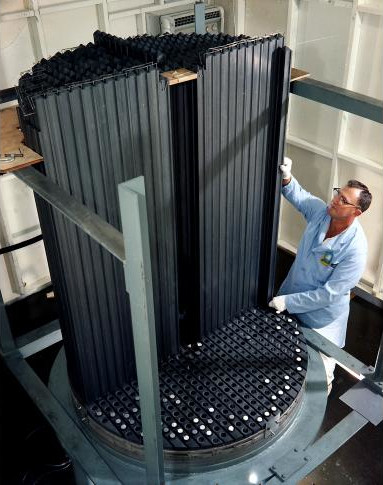
\includegraphics[width=0.4\textwidth]{./references/core-half.jpg}
    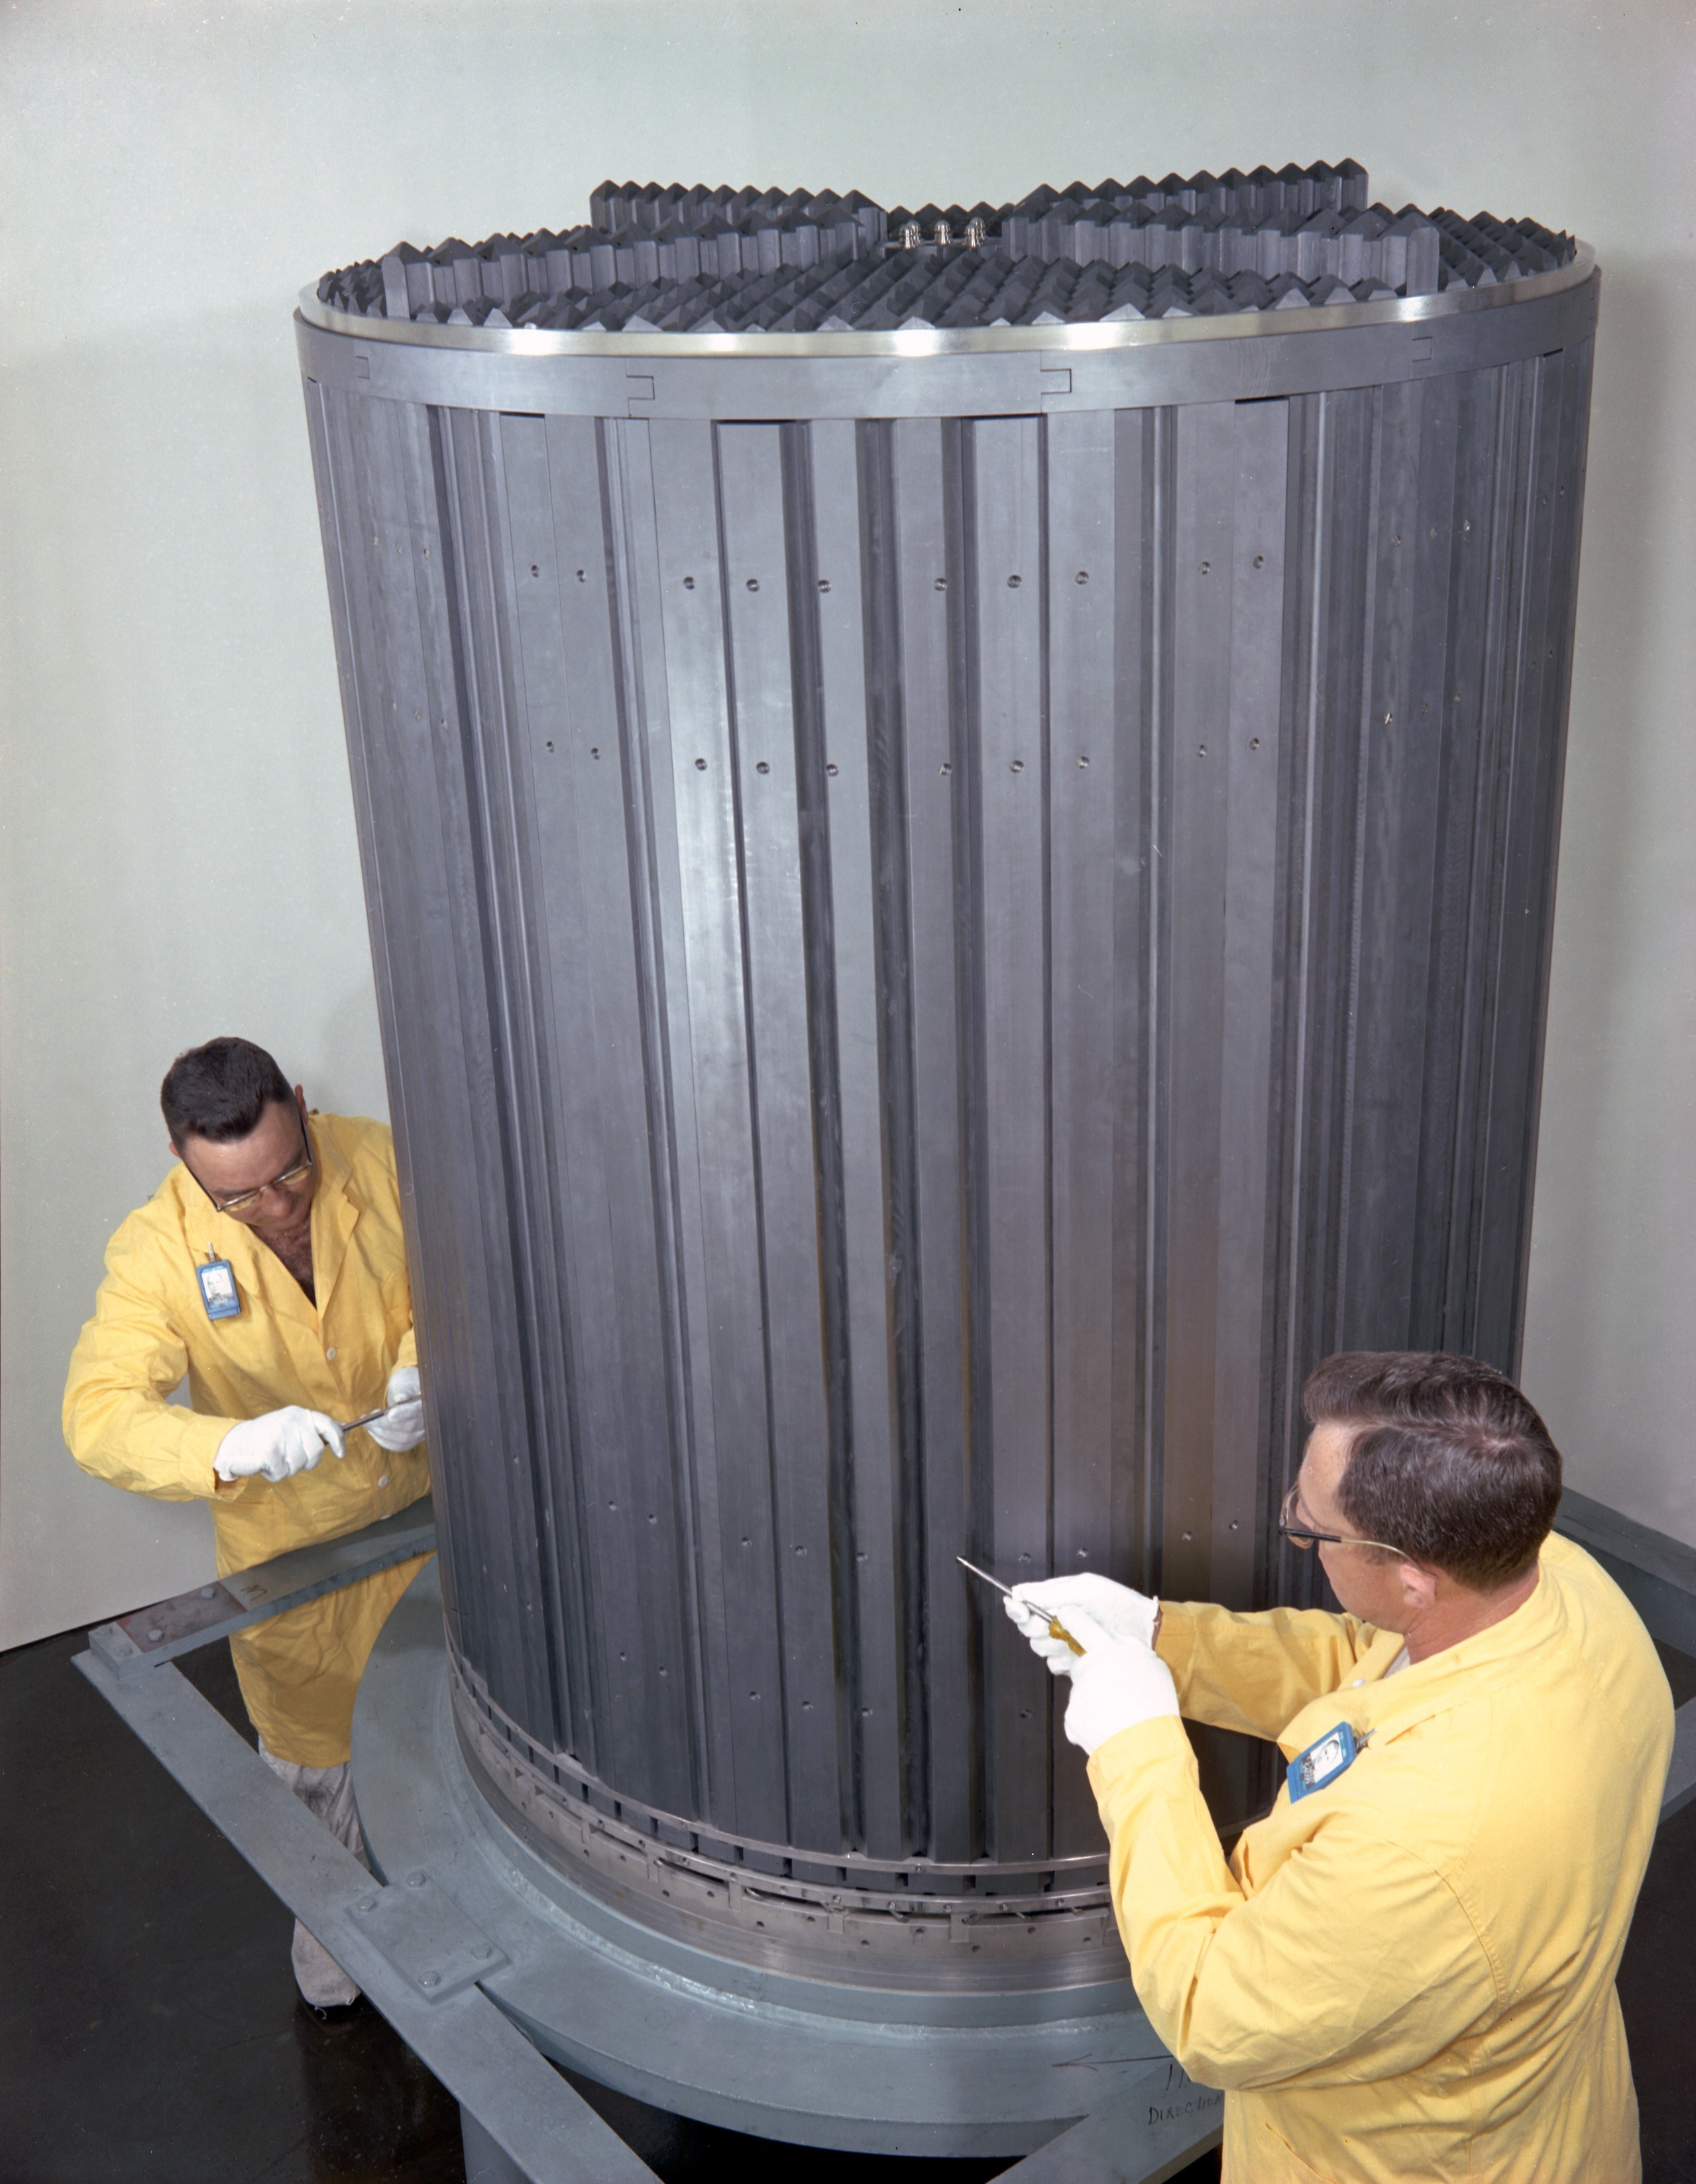
\includegraphics[width=0.393\textwidth]{./references/core-full.jpg}
  }
  \caption{msre graphite core assembly \parencite{ornl}.}
  \label{core-assembly}
\end{figure}
\textcite[page 112 and 114]{ornl-tm-3039} states about the graphite stringers: \enquote{\textit{the reactor core consisted of 617 full and factional sized graphite elements 2x2 in. cross section and about 67 in. long}}. \enquote{\textit{when not buoyed by being immersed in salt, the vertical graphite elements were supported by a lattice of graphite blocks which in turn are supported by a hastelloy-n grid fastened to the bottom of the core can. the core can was thus free to expand downward relative to its top attachment to the reactor vessel while the graphite was free to expand upward relative to its support at the lower end of the core can. the graphite moderator elements were restrained from floating out of core by hastelloy-n rod through holes in the dowel section at the bottom of each graphite element. in addition a wire passing through the upper graphite elements prevented the upper partion of a broken element from floating out of the core}}.

\begin{figure}[H]
  \centering
  \fbox{\includegraphics[page=85,width=0.8\textwidth,trim={4cm 4.8cm 3cm 3cm},clip]{./references/ORNL-3708.pdf}}
  \caption{assembly of graphite bars into msre core \parencite[figure 40]{ornl-3708}.}
  \label{3708-fig40}
\end{figure}

% \begin{figure}[H]
%   \centering
%   \fbox{\includegraphics[page=86,width=0.8\textwidth,trim={4cm 15.5cm 4.6cm 2.9cm},clip]{./references/ORNL-3708.pdf}}
%   \caption{complete graphite core assembly \parencite[figure 41]{ornl-3708}.}
%   \label{3708-fig41}
% \end{figure}

\begin{figure}[H]
  \centering
  \fbox{\includegraphics[page=5,width=0.6\textwidth,trim={7cm 7cm 13cm 19cm},clip]{./references/ORNL-TM-3229.pdf}}
  \caption{zoomed in view of the strainers dowel section, hold-down rods, and core vessel, annulus, and vanes from figure \ref{3229-fig1} \parencite[figure 1]{ornl-tm-3229}. note that the support grid is not depicted here}
\end{figure}
%
\subsection{typical graphite stringer}
a typical graphite stringers, along with a removable graphite stringer, is given in figure \ref{3229-fig2}
\begin{figure}[H]
  \centering
  \centering
  \fbox{\includegraphics[page=6,width=0.8\textwidth,trim={3.5cm 6cm 2.5cm 5cm},clip]{./references/ORNL-TM-3229.pdf}}
  \caption{typical graphite core block arrangement \parencite[figure 2]{ornl-tm-3229}.}
  \label{3229-fig2}
\end{figure}

\textcolor{cyan}{still unknown are the stringers tip taper angle the details on the odd shapped stringers at the edges of the can.}

\textcolor{cyan}{in figure \ref{core-assembly} it seems that the stringers are alligned with metal rods throughout, not to be confused with the support wire at the top (discussed in section \ref{sec:hold-down-rods-support-wires}). whether they stayed in place after assembly and hold the stringers together are not known. neither are the dimensions and locations of these holes.}

\subsubsection{dowels section}
the dowel at the bottom consists of two section dowel (long slim part and stumpy thick part) seen below.
\begin{figure}[H]
  \centering
  \fbox{\includegraphics[page=386,width=0.8\textwidth,trim={2.9cm 6.2cm 3.3cm 4.1cm},clip]{./references/ORNL-3708.pdf}}
  \caption{appearance of spalls and cracks in samples of severly cracked grade cgb graphite in (a) spindle end of a machined bar and (b) midplane of an as-received bar. cracks are indicated by arrows or are clearly visible as ragged white lines. \parencite[figure 4]{ornl-3708}.}
  \label{3708-fig4}
\end{figure}

\begin{itemize}
  \item
  \textcite[page 112 and 114]{ornl-tm-3039} references that the stringers are about 67 in total in length,
  \item
  figure \ref{3229-fig2} indicate that the fuel channel and spike section is 63 in combined,
  \item
  figure \ref{4233-fig2} indicates from the top of the stringer spike to the start of the hold down rod hole is 65 1/2 in in total,
  \item
  figure \ref{core-assembly-zoom} and \ref{0728-p109-p110} indicates that the dowel height is equal to the height of the restrictor ring,
  \item
  \parencite[page 84-85]{ornl-tm-0728} references that the hold down hole rod holes are 0.375 in in diameter,
  \item
  \parencite[page 79 and 81]{ornl-tm-0728} references that the dowel is 1 in in diameter
\end{itemize}
% \parencite[page 84-85]{ornl-tm-0728}.
\textcolor{cyan}{thus, it's assumed that: the dowel disk is 3/4 in in diameter and 1/2 in. in length, the dowel is 1 in. in diameter and 3 1/2 in in length, and the hold-down rod hole is 3 in. from the top of the dowel.}

\subsection{hold-down rods and support wires}
\label{sec:hold-down-rods-support-wires}
\parencite[page 84-85]{ornl-tm-0728} states about the hold-down rods and support wires:
\enquote{\textit{a 5/16-in.-diam inor-8 rod passes through a 0.010-in.-wall-thichness bushing placed in a 0.375-in.-diam hole in the dowel section at the bottom of each graphite stringer. these rods also pass through the inor-8 grid-supporting structure and prevent each graphite stringer from floating in the fuel salt. if a graphite stringer were to break in two, the top partion would tend to float away and leave a relatively stagnant pocket of fuel salt which might reach a higher temperature than desired. the effect of this on the reactivity and on the temperatures in the reactor has been studied. to guard against this eventuality, a 1/16-in.-diam inor-8 wire is passed through a 1/8-in.-diam inor-8 insert about 1 in from the top of each graphite stringer, fastening the tops together and to the core can}}.

figure \ref{0728-p109-p110} gives the orientation of the holes in the stringer hold-down rods relative to the core outlet, that being orthogonal, which is in agreement with figure \ref{3229-fig1}.


\subsection{graphite lattice blocks}
\parencite[page 20]{ornl-tm-3229} states about the lattice blocks: \enquote{\textit{resting on the this}(grid support plates)\textit{ is a grid consisting of two layers of rectangular graphite bars, one layer resting on the other and perpendicular to it. the purpose of the graphite assembly is to position and hold the graphite core blocks, and to compensate for a difference in thermal expansion between the hastelloy n and graphite}}.

\parencite[page 79 and 81]{ornl-tm-0728} states about the lattice blocks: \enquote{\textit{when not buoyed up by being immersed in the fuel salt, the vertical graphite stringers rest on a lattice of graphite blocks, about 1 by 1-5/8 in. in cross section, laid horizontally in two layers at right angles to each other (see ornl dwg. d-bb-b-40420). holes in the lattice blocks, with $4^8-30'$ taper and 1.040 in. in smallest diameter, accept the 1.000-in.-diam doweled section at the lower end of each stringer with sufficient clearance to allow both angular and lateral displacement. the upper horizantal surfaces of the graphite lattice bars and stringers are tapered so that salt will not stand on them after a reactor drain}}.

\begin{figure}[H]
  \centering
  \fbox{
    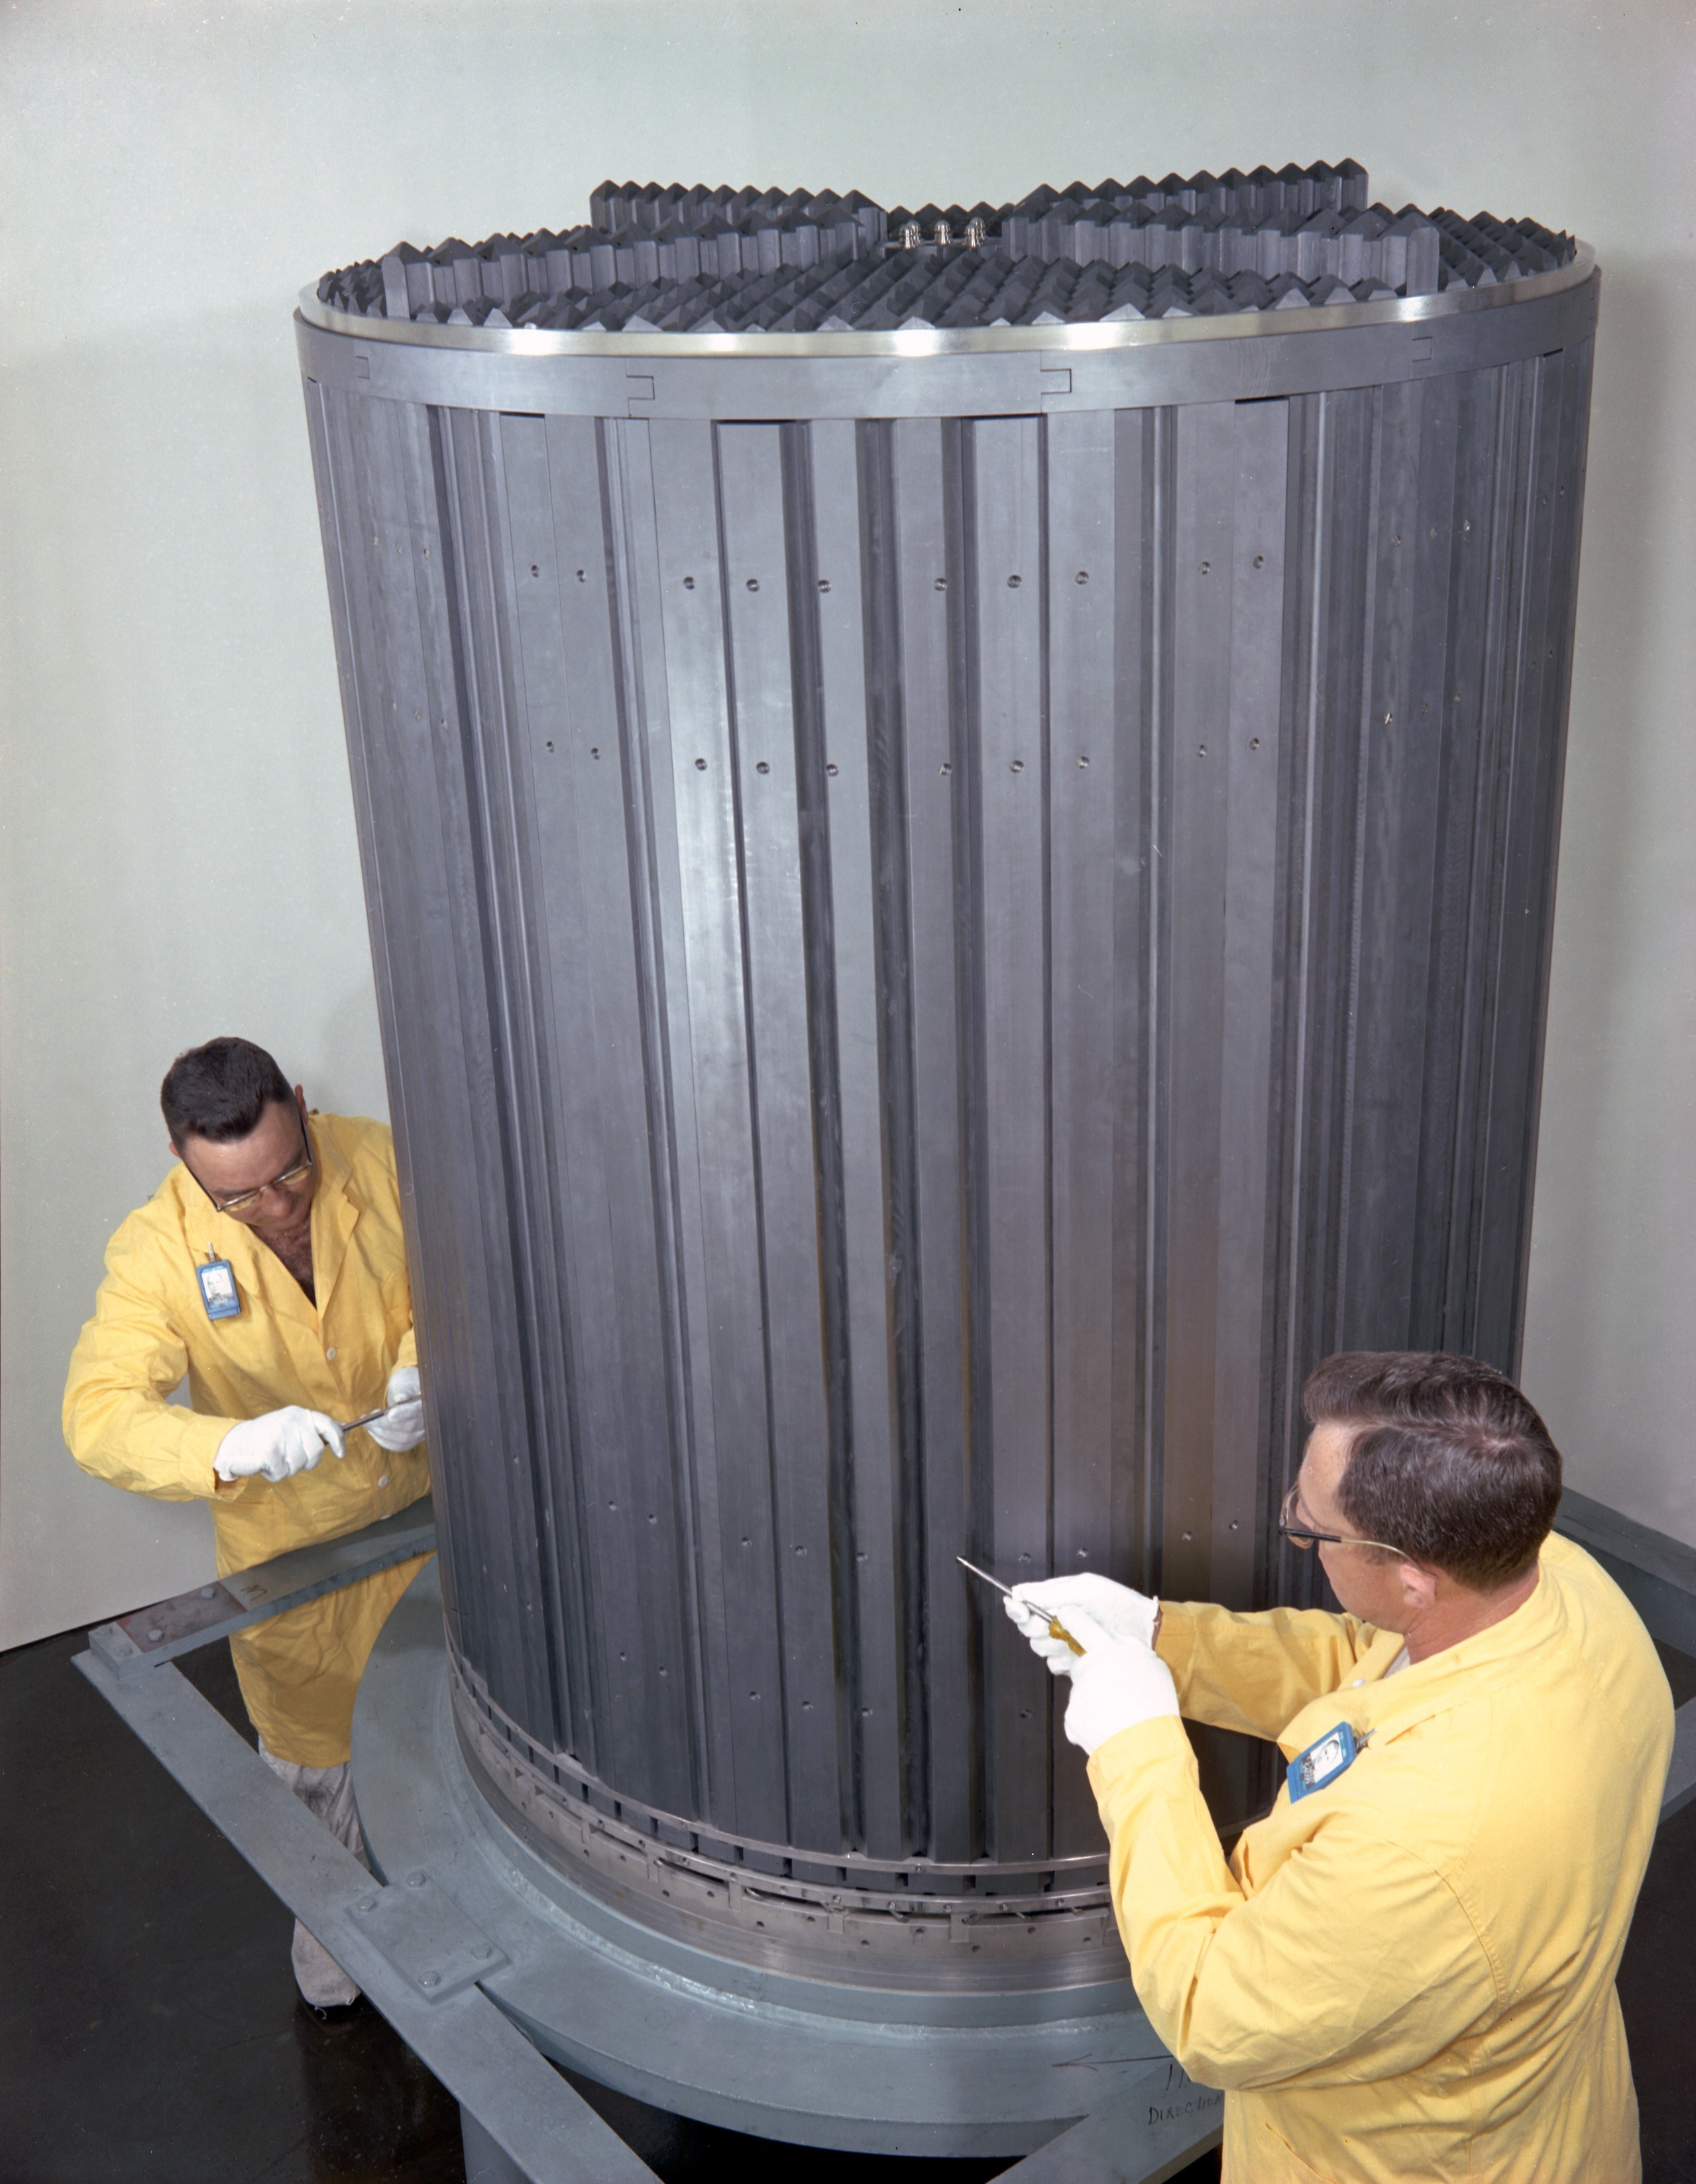
\includegraphics[width=0.8\textwidth,trim={900 300 900 2700},clip]{./references/core-full.jpg}
  }
  \caption{zoomed view of the upper lattice block edges from figure \ref{core-assembly} \parencite{ornl}.}
  \label{core-assembly-zoom}
\end{figure}

\textcolor{cyan}{it can be seen that the graphite stringers sits on top of horizontal graphite lattice blocks, which is also depicted in figure \ref{0728-p109-p110}, but details are lacking.}

\subsection{centering graphite stringers}

\subsection{graphite centering bridge}

\subsection{restrictor ring}
\parencite[page 84-85]{ornl-tm-0728} states about the restrictor ring:
\enquote{\textit{to prevent an excessive amount of salt flow in the annuluar space thus created, an inor-8 restrictor ring, 1/2 x 1/2 x 54-1/2 in. id. surrounds the bundle of graphite stringers at the bottom (see ornl dwg. d-bb-b-40427). the stringers are restrained from excessive movement at the top by a graphite retainer ring, 1 x 2 x 53-1/4 in. id. this ring, in turn, is held in place by an inor-8 retainer ring, 3/4 x 3/4 x 53-1/4 in. id (see ornl dwg. d-bb-b-40428 for both rings). at the top of the graphite blocks a centering bridge holds a row of stringers in position on two diameters at right angles to each other. this bridge helps to prevent shifting of the entire stringer assembly (see ornl dwg. d-bb-b-40424)}}.
\enquote{\textit{the salt leaves the reactor core and flows through the upper head to the 10-in. nozzle opening. it is diverted through a 5-in. opening in the side of the nozzle to flow to the fuel circulating pump. the 10-in. nozzle also serves as an access port and support for the tree control rods and for taking and placing of the four graphite-sample rods in the core matrix. a strainer made from 16-gage inor-8 plate, with a staggered pattern of 3/32-in.-diam holes on 9/64-in. centers, is built into the top head and access plug assembly to prevent large chips of graphite from circulating with the fuel salt}}.




\section{control stringer and sample assembly}
the control stringer and sample assembly is further detailed in figure \ref{61246-fig14a}, \ref{61246-fig14b}, and \ref{61246-fig14c}.
\begin{figure}[H]
  \centering
  \fbox{\includegraphics[page=117,width=0.8\textwidth,trim={2.7cm 5.5cm 3.1cm 4.2cm},clip,angle=0.4]{./references/ORNL-TM-0728.pdf}}
  \caption{lattice arrangement of control rods and sample rod \parencite[figure 5.7]{tm-0728}.}
  \label{0728-fig5-7}
\end{figure}

\parencite[page 81 and 84]{ornl-tm-0728} states about control stringer and sample assembly:
\enquote{\textit{the regular pattern of the graphite stringers in the core is distrupted at the center where the control rod thimbles and the graphite and inor-8 samples are located ... the control rod thimbles are supported from above and the samples are supported from below when no salt is in the reactor}}.
\enquote{\textit{the inor-8 and graphite samples are contained in three baskets in the lattice position ... each basket can be withdrawn independently of the others. a basket must be in place at each of the three locations during reactor operation, however}}.
\enquote{\textit{each basket is formed of 1/32-in.-thick inor-8 plate, perforated with 3/32-in.-diam holes. the top fitting is drilled with 1/8-in.-diam holes on 1/4-in. centers for circulation of the salt and is provided with a t-shaped lifting bail. this bail permits the sample removing tool to rotate as well as lift the basket for better maneuverability. the upper portion of the basket assembly extends from 1-2 to 1-in. into the fuel salt outlet strainer and is held in position by it. the lower end of the basket is provided with an inor-8 fitting, also drilled with 1/8-in. diam holes, which, in conjunction with the other two baskets, forms a dowel to fit into the lower graphite lattice blocks in the same manner as the graphite stringers previously described}}.
\enquote{\textit{each basket contains four 0.250-in.-diam x 5-1/2-ft long samples of inor-8 and five graphite sample bars, 0.250 in. x 0.470 in. ... the graphite bars are devided into samples of varying length (up to about 12 in.), which laid end to end total about 5-1/2 ft. the arrangement of the baskets and contents is experimental in nature and will be varied during operation of the msre}}.
\enquote{\textit{the sample baskets are held down by a cup mounted on a 5/16-in. diam rod which is an extension of the nozzle access plug}}, see figure \ref{0728-p109-p110}.
\enquote{\textit{the cup rests on the t-shaped lifting bails. a thermocouple is installed on the hold-down rod to indicate the salt temperature leaving the reactor}}.


\begin{figure}[H]
  \centering
  \fbox{
    \begin{tabular}{c}
      \includegraphics[page=118,width=0.8\textwidth,trim={10cm 5cm 0cm 4cm},clip,angle=-90]{./references/ORNL-TM-0728.pdf} \\ [-0.3cm]
      \includegraphics[page=119,height=0.5\textwidth,trim={0cm 4.15cm 7cm 3cm},clip,angle=-90]{./references/ORNL-TM-0728.pdf}
    \end{tabular}
  }
  \caption{graphite-inor-8 sample assembly \parencite[figure 5.8]{tm-0728}.}
  \label{0728-fig5-8}
\end{figure}

\parencite[page 84]{ornl-tm-0728} states about the center stringers:
\enquote{\textit{in addition to the graphite samples in the baskets, the five graphite stringers at the center of the core can be removed, although with considerable more difficulty}}, the location of these stringers is indicated in figure \ref{0728-fig5-7}.
\enquote{\textit{the five stringers are of a special design (types 7, 60, and 61 on ornl dwgs d-bb-b-40416, 40418 and 40581). they are 2-in. x 2-in. in cross section but are 64-1/2 in. long rather than the 62-1/8 in. of the average stringer. they do not have the dowel section at the bottom and the hole for the hold-down rods and they rest directly on the inor-8 supporting grid rather than on the graphite lattice blocks. the lattice blocks do not extend across the five stringer locations, the opening thus provided through the blocks permitting insertion of a viewing device through the core to permit observation of the lower head should this prove desirable.}}


\begin{figure}[H]
  \centering
  \fbox{\includegraphics[page=23,width=0.8\textwidth,trim={4cm 2cm 4.8cm 2cm},clip]{./references/AD-CF-61-2-46.pdf}}
  \caption{msre control stringer arrangement \parencite[figure 14a]{ad-cf-61-2-46}.}
  \label{61246-fig14a}
\end{figure}

\begin{figure}[H]
  \centering
  \fbox{\includegraphics[page=24,width=0.8\textwidth,trim={2.5cm 2cm 2.5cm 2.5cm},clip]{./references/AD-CF-61-2-46.pdf}}
  \caption{vertical section-poison control stringer \parencite[figure 14b]{ad-cf-61-2-46}.}
  \label{61246-fig14b}
\end{figure}

\begin{figure}[H]
  \centering
  \fbox{\includegraphics[page=8,width=0.8\textwidth,trim={6cm 15cm 7cm 3cm},clip]{./references/ORNL-4123.pdf}}
  \caption{cutaway of an msre control element \parencite[figure 1]{ornl-4123}.}
  \label{4123-fig1}
\end{figure}

\begin{figure}[H]
  \centering
  \fbox{
    \begin{tabular}{c}
        \includegraphics[page=43,width=0.4\textwidth,trim={4cm 16.5cm 4cm 2cm},clip]{./references/ORNL-4123.pdf} \\
        \includegraphics[page=43,width=0.4\textwidth,trim={4cm 5.5cm 4cm 16cm},clip]{./references/ORNL-4123.pdf}
    \end{tabular}
    \begin{tabular}{c}
        \includegraphics[page=44,width=0.4\textwidth,trim={4cm 7cm 4cm 12cm},clip]{./references/ORNL-4123.pdf} \\
        \includegraphics[page=44,width=0.4\textwidth,trim={4cm 19.5cm 4cm 2.5cm},clip]{./references/ORNL-4123.pdf}
    \end{tabular}
  }
  \caption{control element assembly \parencite[figure B-1 to B-4]{ornl-4123}.}
  \label{4123-fig1}
\end{figure}

\begin{figure}[H]
  \centering
  \centering
  \fbox{\includegraphics[page=130,width=0.8\textwidth,trim={3.8cm 3.7cm 3.5cm 2.5cm},clip,angle=0.25]{./references/ORNL-TM-3039.pdf}}
  \caption{msre surveillance facility inside reactor vessel \parencite[figure 5.14]{ornl-tm-3229}.}
  \label{3039-fig5-11}
\end{figure}

\subsection{removable graphite stringer}
\parencite[page 84]{ornl-tm-0728} states about the removable graphite stringer:
\enquote{\textit{the five graphite stringers at the center of the core can be removed, although with considerable more difficulty}}. see figure \ref{0728-fig5-7}. \enquote{\textit{the five stringers are of a special design (types 7, 60 and 61 on ornl dwgs d-bb-b-40416, 40418 and 40581). they are 2-in. x 2-in. in cross section but are 64-1/2 in. long rather than the 62-1/8 in. of the average stringer. they do not have the dowel section at the bottom and the hole for the hold-down rods and they rest directly on the inor-8 supporting grid rather than on the graphite lattice blocks. the lattice blocks do not extend across the five stringers locations, the opening thus provided through the blocks permitting insertion of a viewing device through the core to permit observation of the lower head should this prove desirable}}.
\enquote{\textit{each of the five stringers is drilled and tapped with a 3/4-in. 6 acme thread on the upper end for an inor-8 lifting knob, or stud, which can engage a snaptite quick-disconnect coupling. they are prevented from floating in the fuel salt by 1/8 in. x 1/2 in. hold-down bars welded to the strainer assembly at a level even with the top of the graphite core. (see ornl dwg e-bb-b-40598)}}. see the figure \ref{3229-fig2}.






\printbibliography

\end{preview}
\end{document}


% \begin{table}[H]
%   \centering
%   \caption{properties of msre core graphite \parencite[table 3]{ad-cf-61-2-46}.}
%   \fbox{\includegraphics[page=9,width=0.8\textwidth,trim={2cm 4cm 2cm 3.4cm},clip]{./references/AD-CF-61-2-46.pdf}}
%   \label{61246-tab3}
% \end{table}
